\documentclass[10pt,aspectratio=169]{beamer}
\usetheme{Madrid}
\setbeamertemplate{navigation symbols}{}

\usepackage{booktabs}
\usepackage{graphicx}
\usepackage{multicol}
\usepackage{array}

\title[Fraud Detection with XGBoost]{CREDIT CARD FRAUD DETECTION USING\\EXTREME GRADIENT BOOSTING}
\author[Dai, Dang, Huy]{Nguyen Trong Dai \and Mai Huy Dang \and Vu Quoc Huy}
\institute{AI66A Group 1}
\date{\today}

\begin{document}

\begin{frame}
  \titlepage
\end{frame}

\begin{frame}{Problem and Goal}
  \begin{itemize}
    \item Fraud is rare but high-impact: only around 0.5\% of transactions are fraudulent.
    \item A model can get very high accuracy while still missing most fraud cases.
    \item Main objective: maximize fraud detection while keeping false alerts low.
    \item Priority metrics:
      \begin{itemize}
        \item Recall (catch fraud)
        \item F2-score (recall weighted 2x more than precision)
        \item PR-AUC (best metric for imbalanced classification)
      \end{itemize}
  \end{itemize}
\end{frame}

\begin{frame}{Dataset Overview}
  \begin{columns}[T]
    \column{0.48\textwidth}
    \small
    \begin{tabular}{lrrr}
      \toprule
      Split & Transactions & Fraud & Rate \\
      \midrule
      Train & 1,296,675 & 7,506 & 0.579\% \\
      Test  & 555,719   & 2,145 & 0.386\% \\
      \bottomrule
    \end{tabular}

    \vspace{0.5em}
    \begin{itemize}
      \item Source: Kaggle credit card fraud dataset.
      \item 23 raw columns (time, amount, location, merchant, user attributes).
      \item No missing values and no duplicate transactions.
    \end{itemize}

    \column{0.48\textwidth}
    \centering
    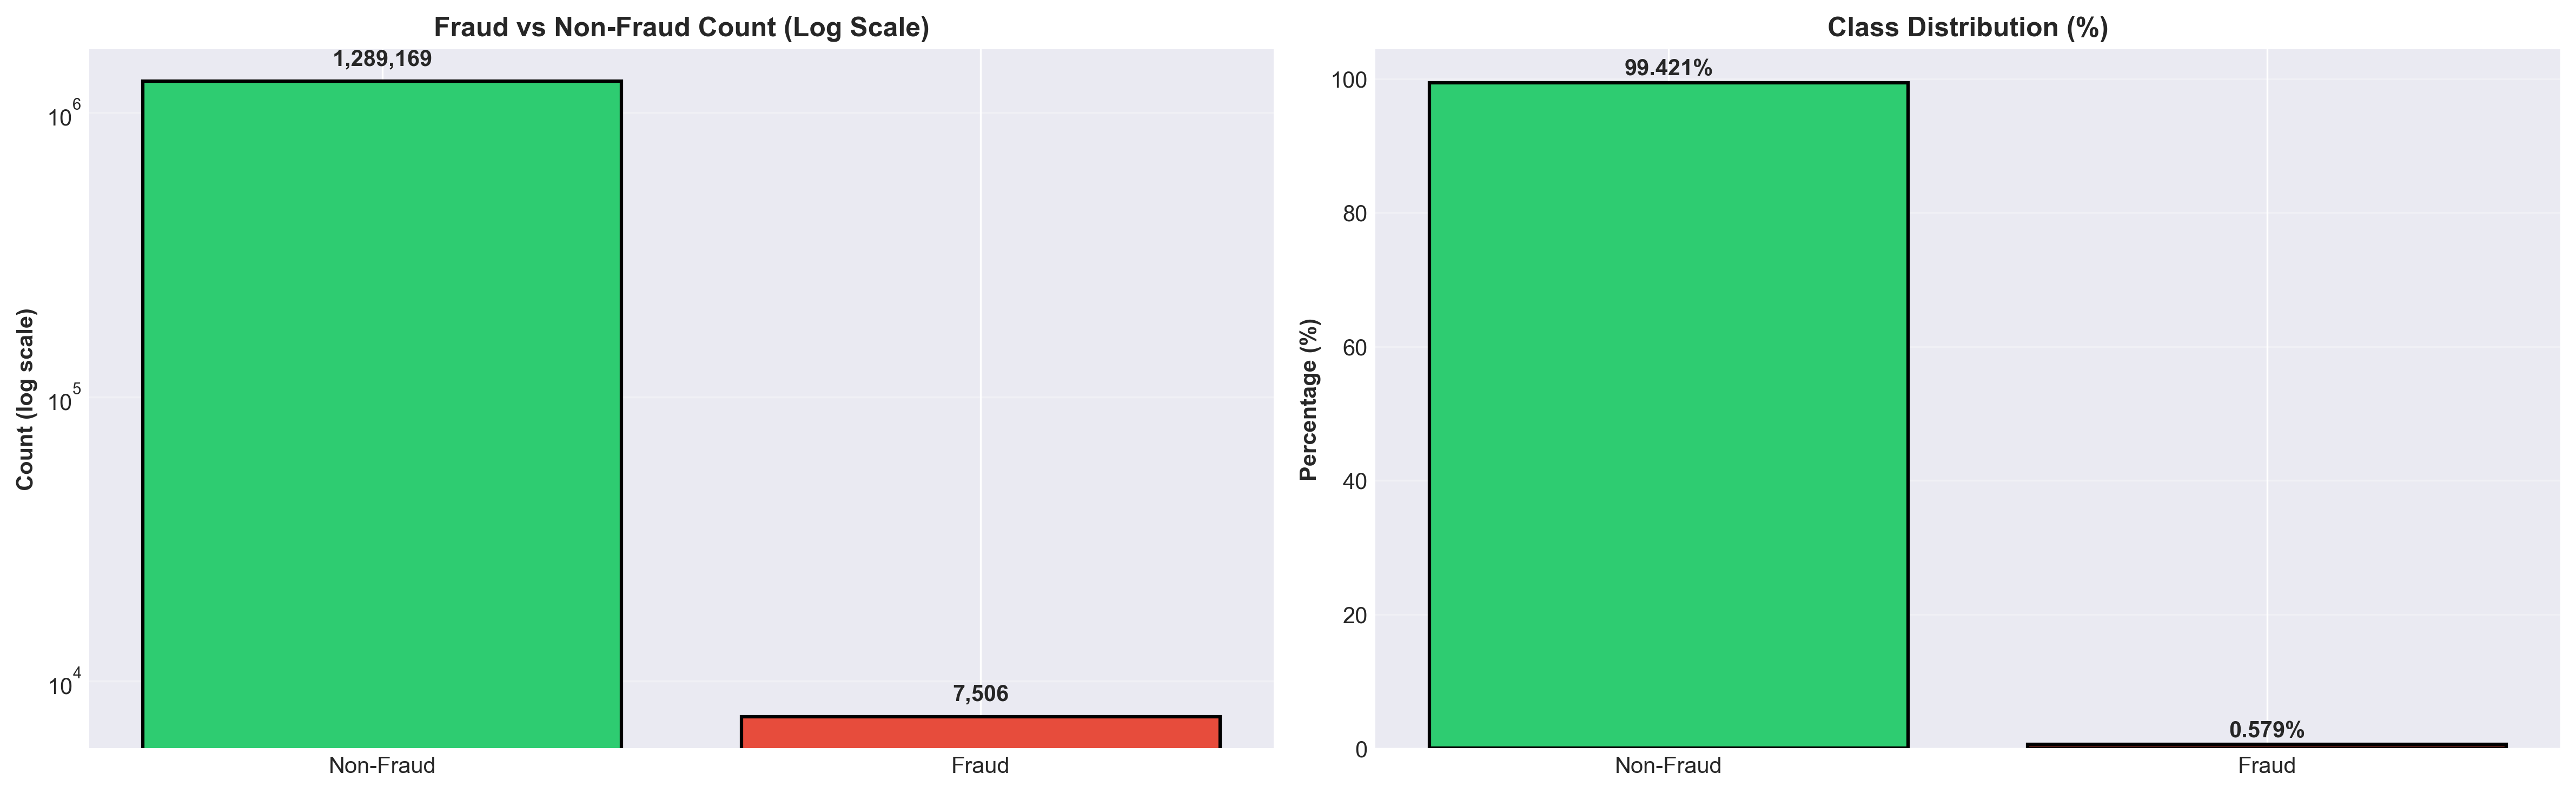
\includegraphics[width=\linewidth]{images/fraud_distribution.png}
  \end{columns}
\end{frame}

\begin{frame}{Data Quality and Leakage Control}
  \begin{columns}[T]
    \column{0.52\textwidth}
    \begin{itemize}
      \item Outliers in \texttt{amt} were kept because they carry real fraud signal.
      \item \texttt{trans\_date\_trans\_time} was dropped after extracting time features.
      \item Target encoding used out-of-fold estimation (StratifiedKFold, k=5).
      \item Unseen categories in test data are mapped to global fraud rate.
      \item This prevents target leakage from test into training.
    \end{itemize}
    \column{0.44\textwidth}
    \centering
    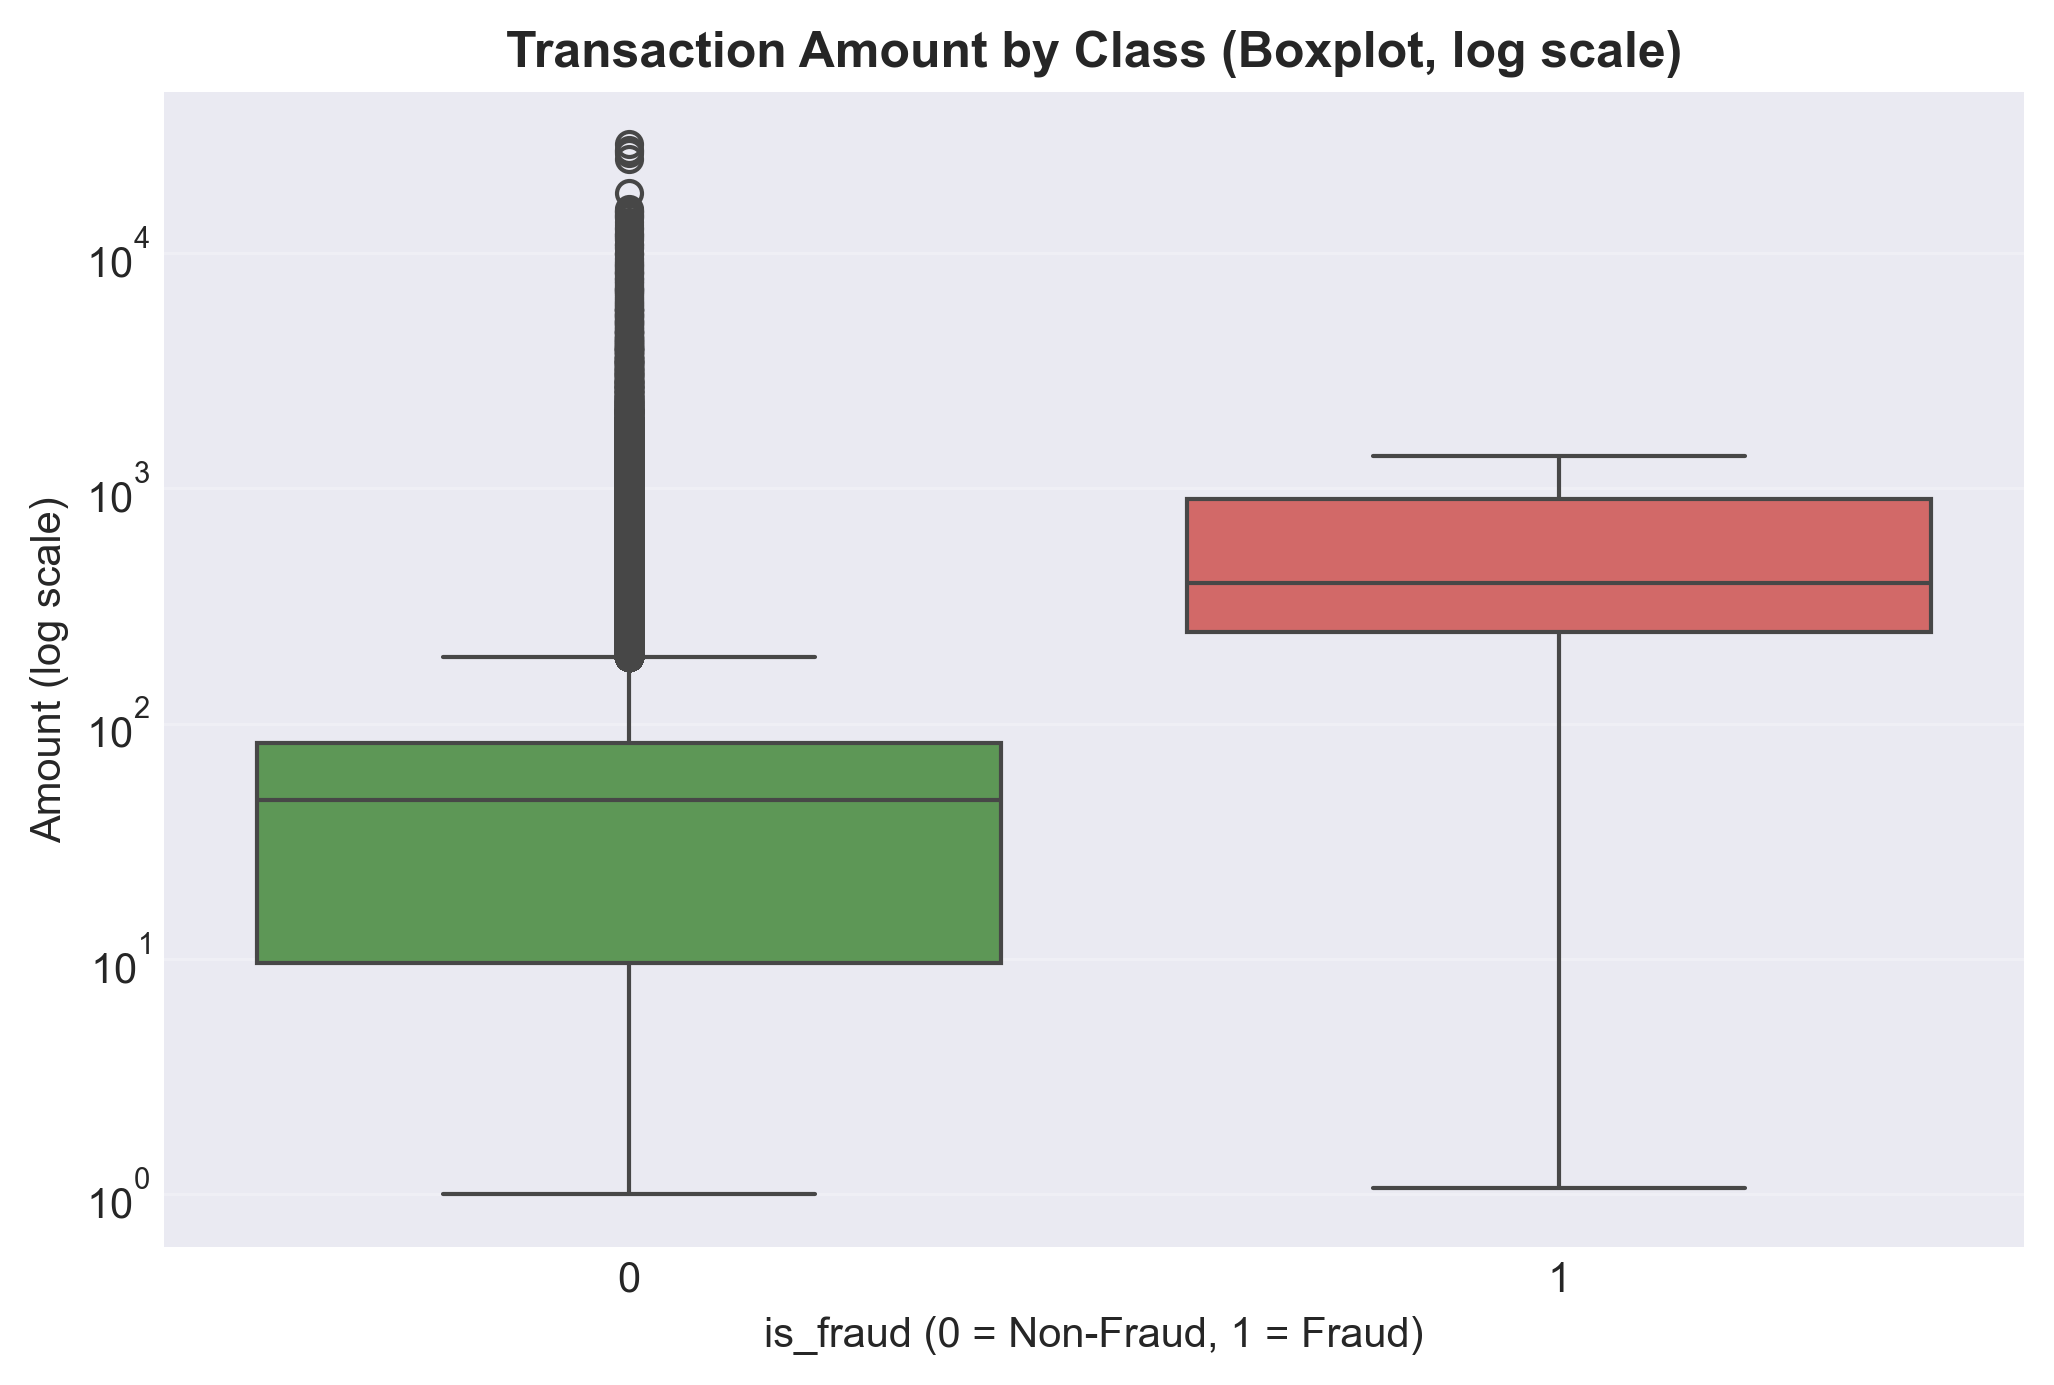
\includegraphics[width=\linewidth]{images/transaction_amount.png}
  \end{columns}
\end{frame}

\begin{frame}{Feature Engineering}
  \small
  \begin{columns}[T]
    \column{0.49\textwidth}
    \textbf{Engineered features}
    \begin{itemize}
      \item Time: \texttt{hour}, \texttt{day\_of\_week}, \texttt{month}, \texttt{is\_weekend}, \texttt{is\_night}
      \item Amount transforms: \texttt{amt\_log}, \texttt{amt\_zscore}
      \item User age: \texttt{age}
      \item Geo distance: \texttt{distance\_km}
      \item Frequency encodings: category, merchant, city
      \item Target encodings: category, merchant, city fraud rates
    \end{itemize}

    \column{0.49\textwidth}
    \textbf{Final 9 features used}
    \begin{multicols}{2}
    \begin{itemize}
      \item amt
      \item hour
      \item age
      \item city\_pop
      \item gender
      \item category\_freq
      \item merchant\_freq
      \item category fraud rate
      \item merchant fraud rate
    \end{itemize}
    \end{multicols}

    \textbf{Notable finding:} dropping \texttt{city\_fraud\_rate} improved recall/F2 by about 30--40 points.
  \end{columns}
\end{frame}

\begin{frame}{Feature Selection Evidence}
  \begin{columns}[T]
    \column{0.48\textwidth}
    \begin{itemize}
      \item SHAP explains feature contribution at transaction level.
      \item Permutation importance validates whether a feature helps global performance.
      \item Features with near-zero or negative importance were removed.
      \item Harmful features removed:
      \begin{itemize}
        \item \texttt{city\_fraud\_rate} (around -0.36)
        \item \texttt{is\_night} (negative effect)
      \end{itemize}
    \end{itemize}
    \column{0.48\textwidth}
    \centering
    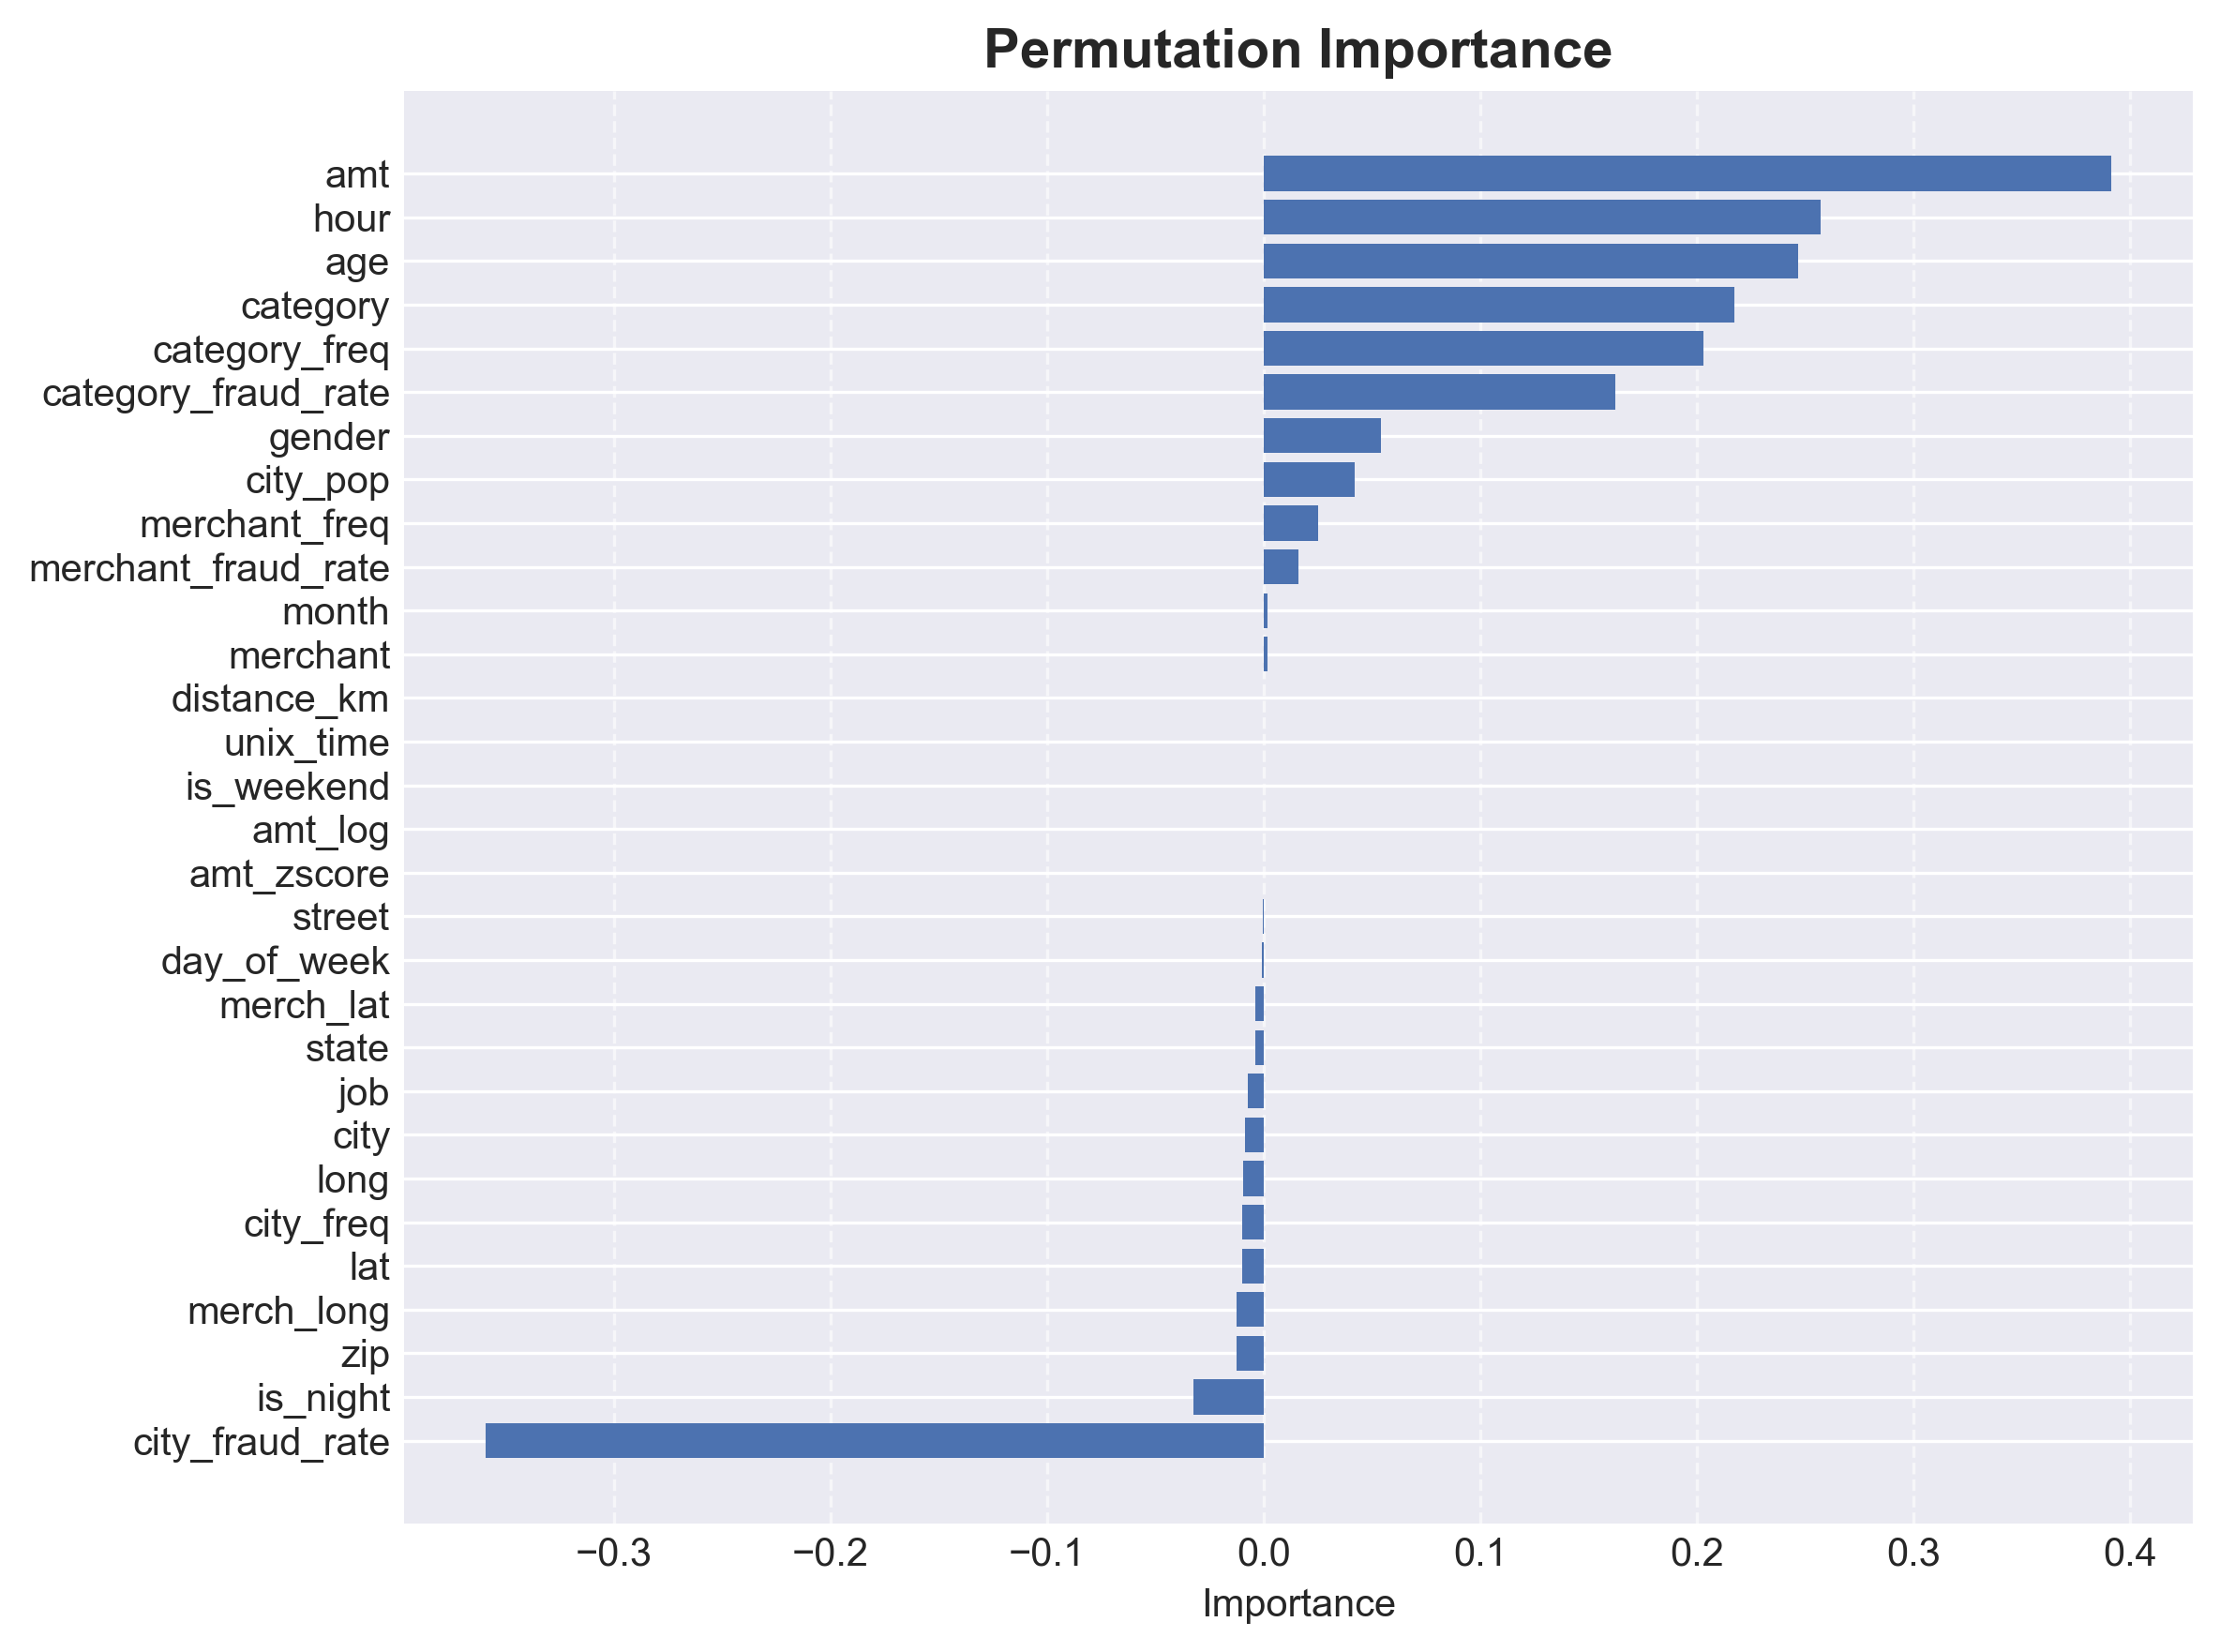
\includegraphics[width=\linewidth]{images/permutation_importance.png}
  \end{columns}
\end{frame}

\begin{frame}{Modeling Approach}
  \small
  \begin{itemize}
    \item Evaluated 5 models on the same feature set:
      \begin{itemize}
        \item Logistic Regression (baseline)
        \item Random Forest
        \item LightGBM
        \item XGBoost
        \item MLP (PyTorch)
      \end{itemize}
    \item Class imbalance handled by \texttt{scale\_pos\_weight = 171.75}.
    \item XGBoost chosen for best overall trade-off among PR-AUC, recall, F2, and false alerts.
    \item Hyperparameter optimization: Optuna (TPE), 50 trials, objective = PR-AUC.
  \end{itemize}
\end{frame}

\begin{frame}{Imbalance Handling Comparison}
  \small
  \begin{tabular}{lccccc}
    \toprule
    Strategy & Precision & Recall & F2 & PR-AUC & False Alerts \\
    \midrule
    \texttt{scale\_pos\_weight} & \textbf{65.6\%} & 86.2\% & \textbf{0.8115} & \textbf{0.8871} & \textbf{969} \\
    Undersampling & 27.68\% & 95.34\% & 0.6403 & 0.8856 & 5,344 \\
    SMOTE & 6.52\% & \textbf{96.04\%} & 0.2564 & 0.8378 & 29,536 \\
    \bottomrule
  \end{tabular}

  \vspace{0.7em}
  \begin{itemize}
    \item \texttt{scale\_pos\_weight} gave the best balance without modifying original data distribution.
    \item Resampling raised recall but produced too many false alerts.
  \end{itemize}
\end{frame}

\begin{frame}{Evaluation and Threshold Strategy}
  \begin{itemize}
    \item Accuracy is excluded due to severe class imbalance.
    \item Core metrics:
      \begin{itemize}
        \item Recall: minimize missed fraud (FN)
        \item F2-score: optimize recall with precision control
        \item PR-AUC: model selection and Optuna objective
      \end{itemize}
    \item Threshold optimization performed on Precision-Recall curve.
    \item Default threshold 0.5 was replaced by F2-optimized threshold 0.9534.
    \item Result: precision improved strongly while recall stayed high.
  \end{itemize}
\end{frame}

\begin{frame}{Final Model Performance}
  \begin{columns}[T]
    \column{0.46\textwidth}
    \small
    \textbf{Tuned XGBoost + threshold 0.9534}
    \vspace{0.4em}

    \begin{tabular}{lr}
      \toprule
      Metric & Value \\
      \midrule
      PR-AUC & 0.8975 \\
      ROC-AUC & 0.9978 \\
      Precision & 76.2\% \\
      Recall & 85.0\% \\
      F2-score & 0.8311 \\
      False Alert Rate & 0.10\% \\
      \bottomrule
    \end{tabular}

    \vspace{0.4em}
    \begin{itemize}
      \item TP: 1,824
      \item FP: 570
      \item FN: 321
      \item TN: 553,004
    \end{itemize}

    \column{0.50\textwidth}
    \centering
    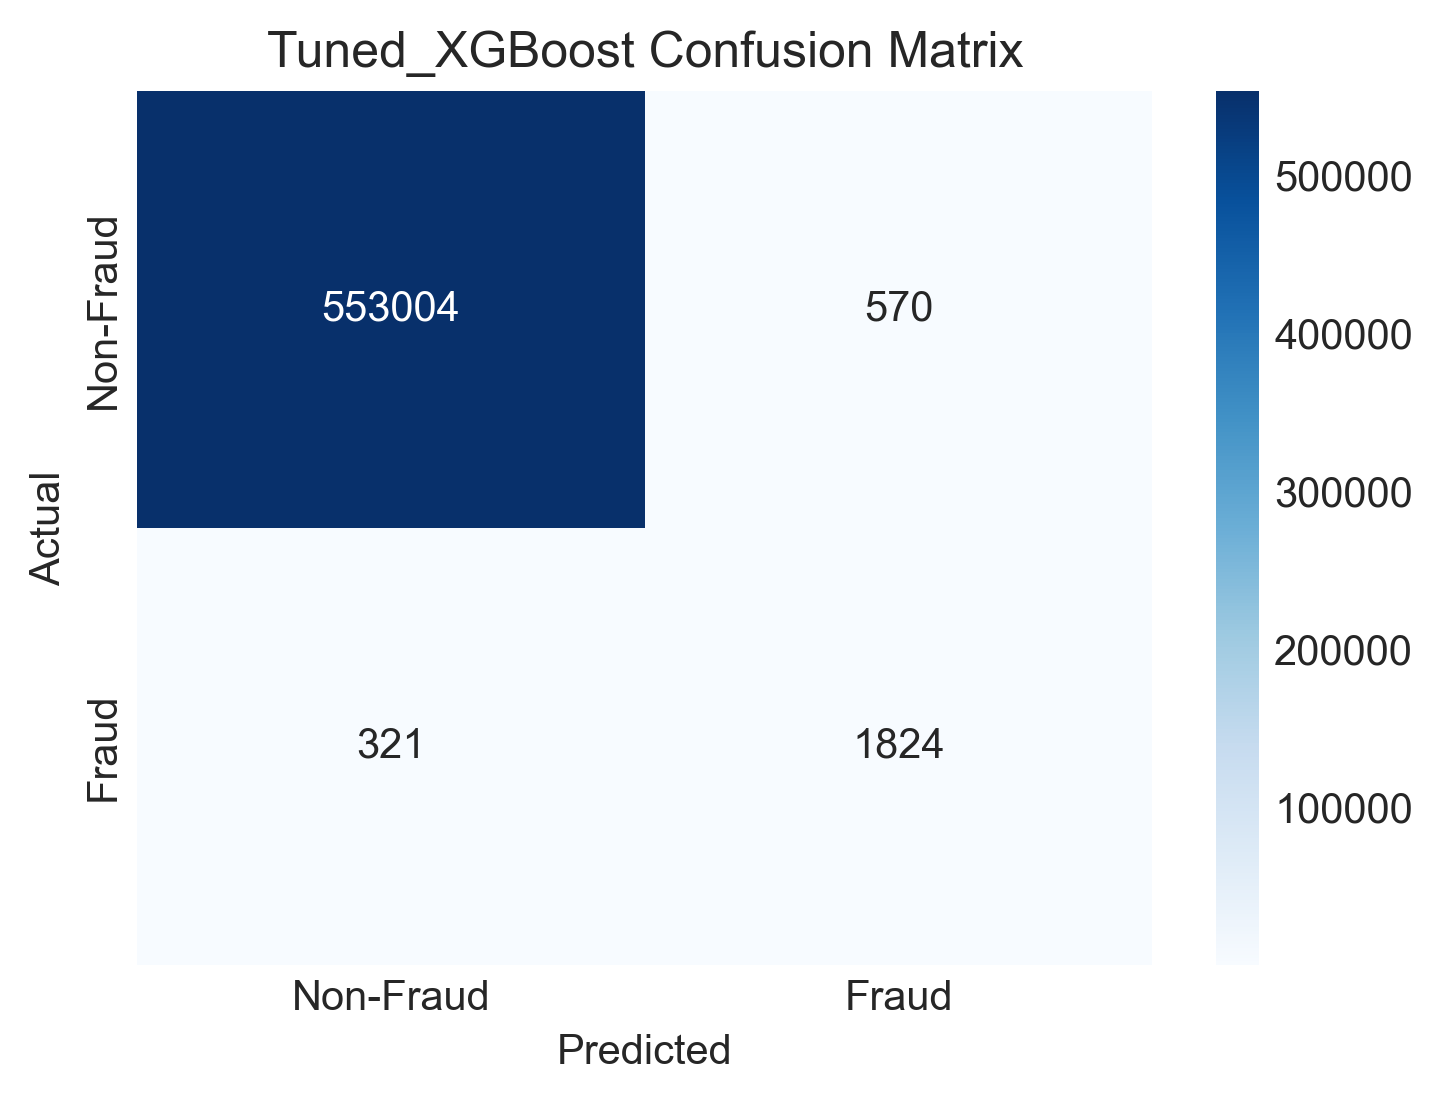
\includegraphics[width=\linewidth]{images/Tuned_XGBoost_confusion_matrix.png}
  \end{columns}
\end{frame}

\begin{frame}{Baseline vs Tuned XGBoost}
  \begin{columns}[T]
    \column{0.49\textwidth}
    \small
    \begin{tabular}{lcc}
      \toprule
      Metric & Baseline & Tuned \\
      \midrule
      PR-AUC & 0.8872 & 0.8975 \\
      Precision & 65.63\% & 76.2\% \\
      Recall & 86.25\% & 85.0\% \\
      F2-score & 0.8115 & 0.8311 \\
      False Alert Rate & 0.175\% & 0.10\% \\
      \bottomrule
    \end{tabular}

    \vspace{0.6em}
    \begin{itemize}
      \item Precision: +10.57 points
      \item F2-score: +0.0196
      \item False alert rate: down by 0.075 points
    \end{itemize}

    \column{0.49\textwidth}
    \centering
    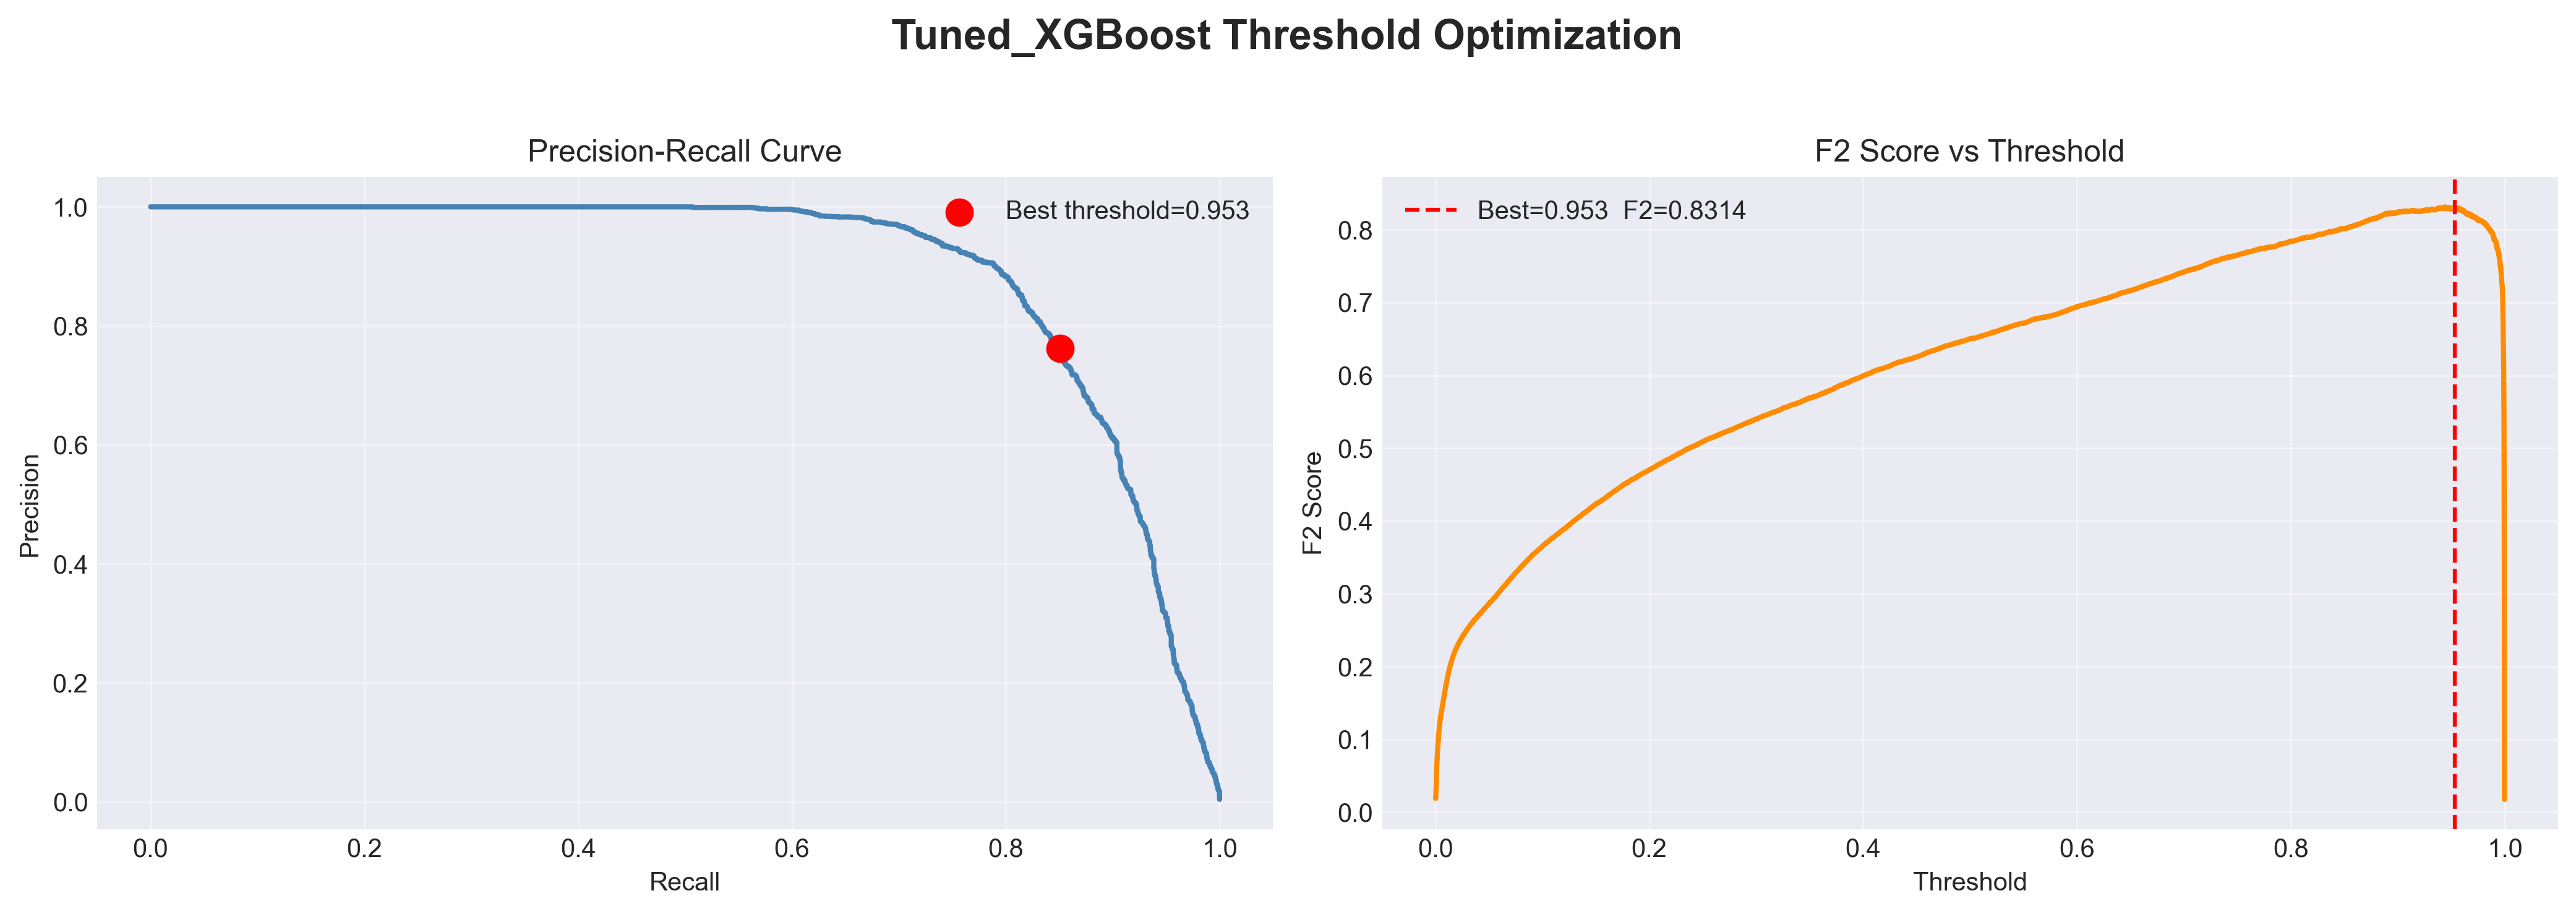
\includegraphics[width=\linewidth]{images/Tuned_XGBoost_optimization.png}
  \end{columns}
\end{frame}

\begin{frame}[t]{Model Explainability}
  \begin{columns}[T]
    \column{0.56\textwidth}
    \centering
    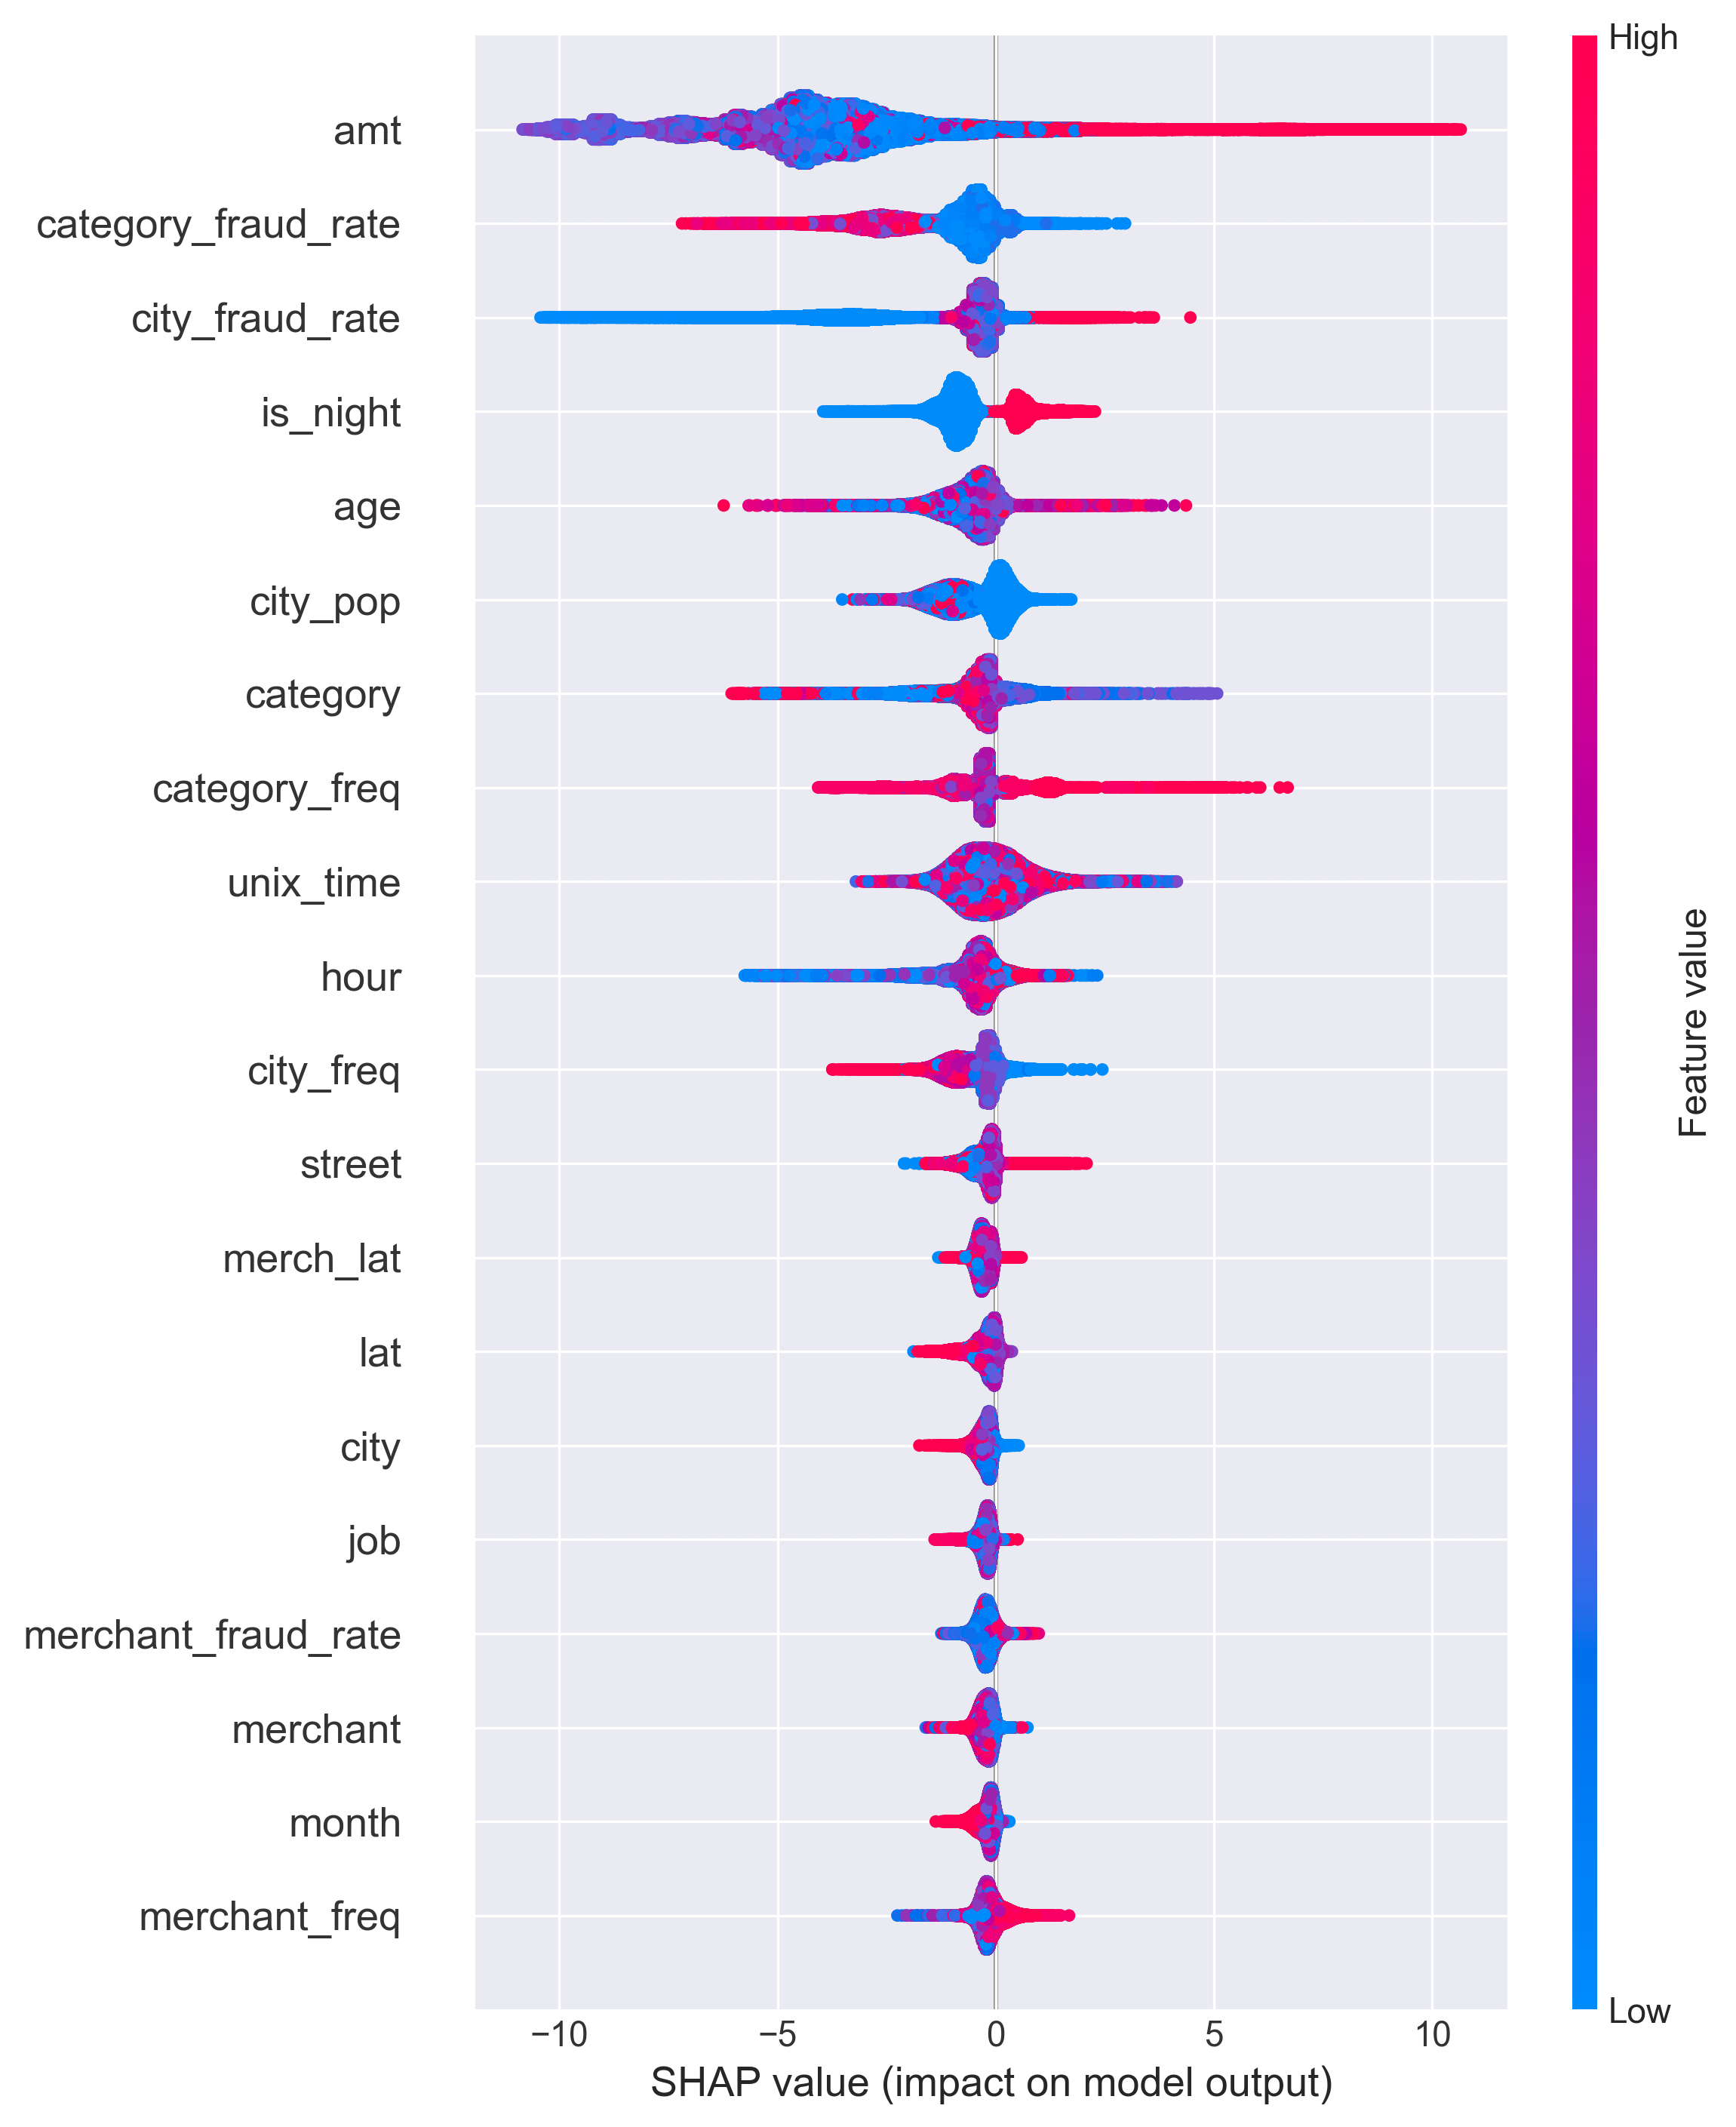
\includegraphics[height=0.55\textheight,keepaspectratio]{images/shap_summary.png}
    \column{0.40\textwidth}
    \footnotesize
    \textbf{Main insights}
    \begin{itemize}
      \item \texttt{amt} is the strongest fraud signal.
      \item Category fraud rate and \texttt{hour} are key drivers.
      \item SHAP + permutation helped remove harmful features.
    \end{itemize}
  \end{columns}
\end{frame}

\begin{frame}{Deployment Plan}
  \small
  \textbf{Saved artifacts}
  \begin{itemize}
    \item \texttt{models/xgb\_fraud\_final.pkl}
    \item \texttt{models/model\_metadata.json} (feature order, threshold, metrics, params)
  \end{itemize}

  \textbf{Inference contract}
  \begin{itemize}
    \item Input must contain the 9 engineered features in correct order.
    \item Output includes \texttt{fraud\_probability} and \texttt{is\_fraud\_predicted}.
  \end{itemize}

  \textbf{Path to production}
  \begin{itemize}
    \item REST API (FastAPI/Flask)
    \item Feature store for live encodings
    \item Model registry and versioning
    \item Drift monitoring and scheduled retraining
  \end{itemize}
\end{frame}

\begin{frame}{Conclusion}
  \begin{itemize}
    \item XGBoost is the best model for this tabular fraud detection task.
    \item Final system catches 85\% fraud with 76.2\% precision and only 0.10\% false alerts.
    \item Strongest gains came from:
      \begin{itemize}
        \item robust feature selection
        \item proper imbalance handling
        \item F2-based threshold optimization
      \end{itemize}
    \item This pipeline is a solid baseline for real-time fraud detection deployment.
  \end{itemize}
\end{frame}

\end{document}
